\section{\uppercase{Design and Architecture}}
\label{sec:architecture}

% principles
\noindent Workflow and requirements described in the previous section have been received in \emph{Metior}, a prototypal application serving as proof of concept. With the aim of maximize accessibility for surveyors, it is strongly web based and runs in modern browsers. it is built using React by Facebook and an MVC design pattern with \emph{unidirectional data flow} \cite{redux}:  it ensures the best code maintainability and debuggability by centralizing access to the application state to a single controller.

\subsection{UI \& UX}

The web application appears as a simplified CAD.

\begin{figure}[htbp] %  figure placement: here, top, bottom, or page
   \centering

   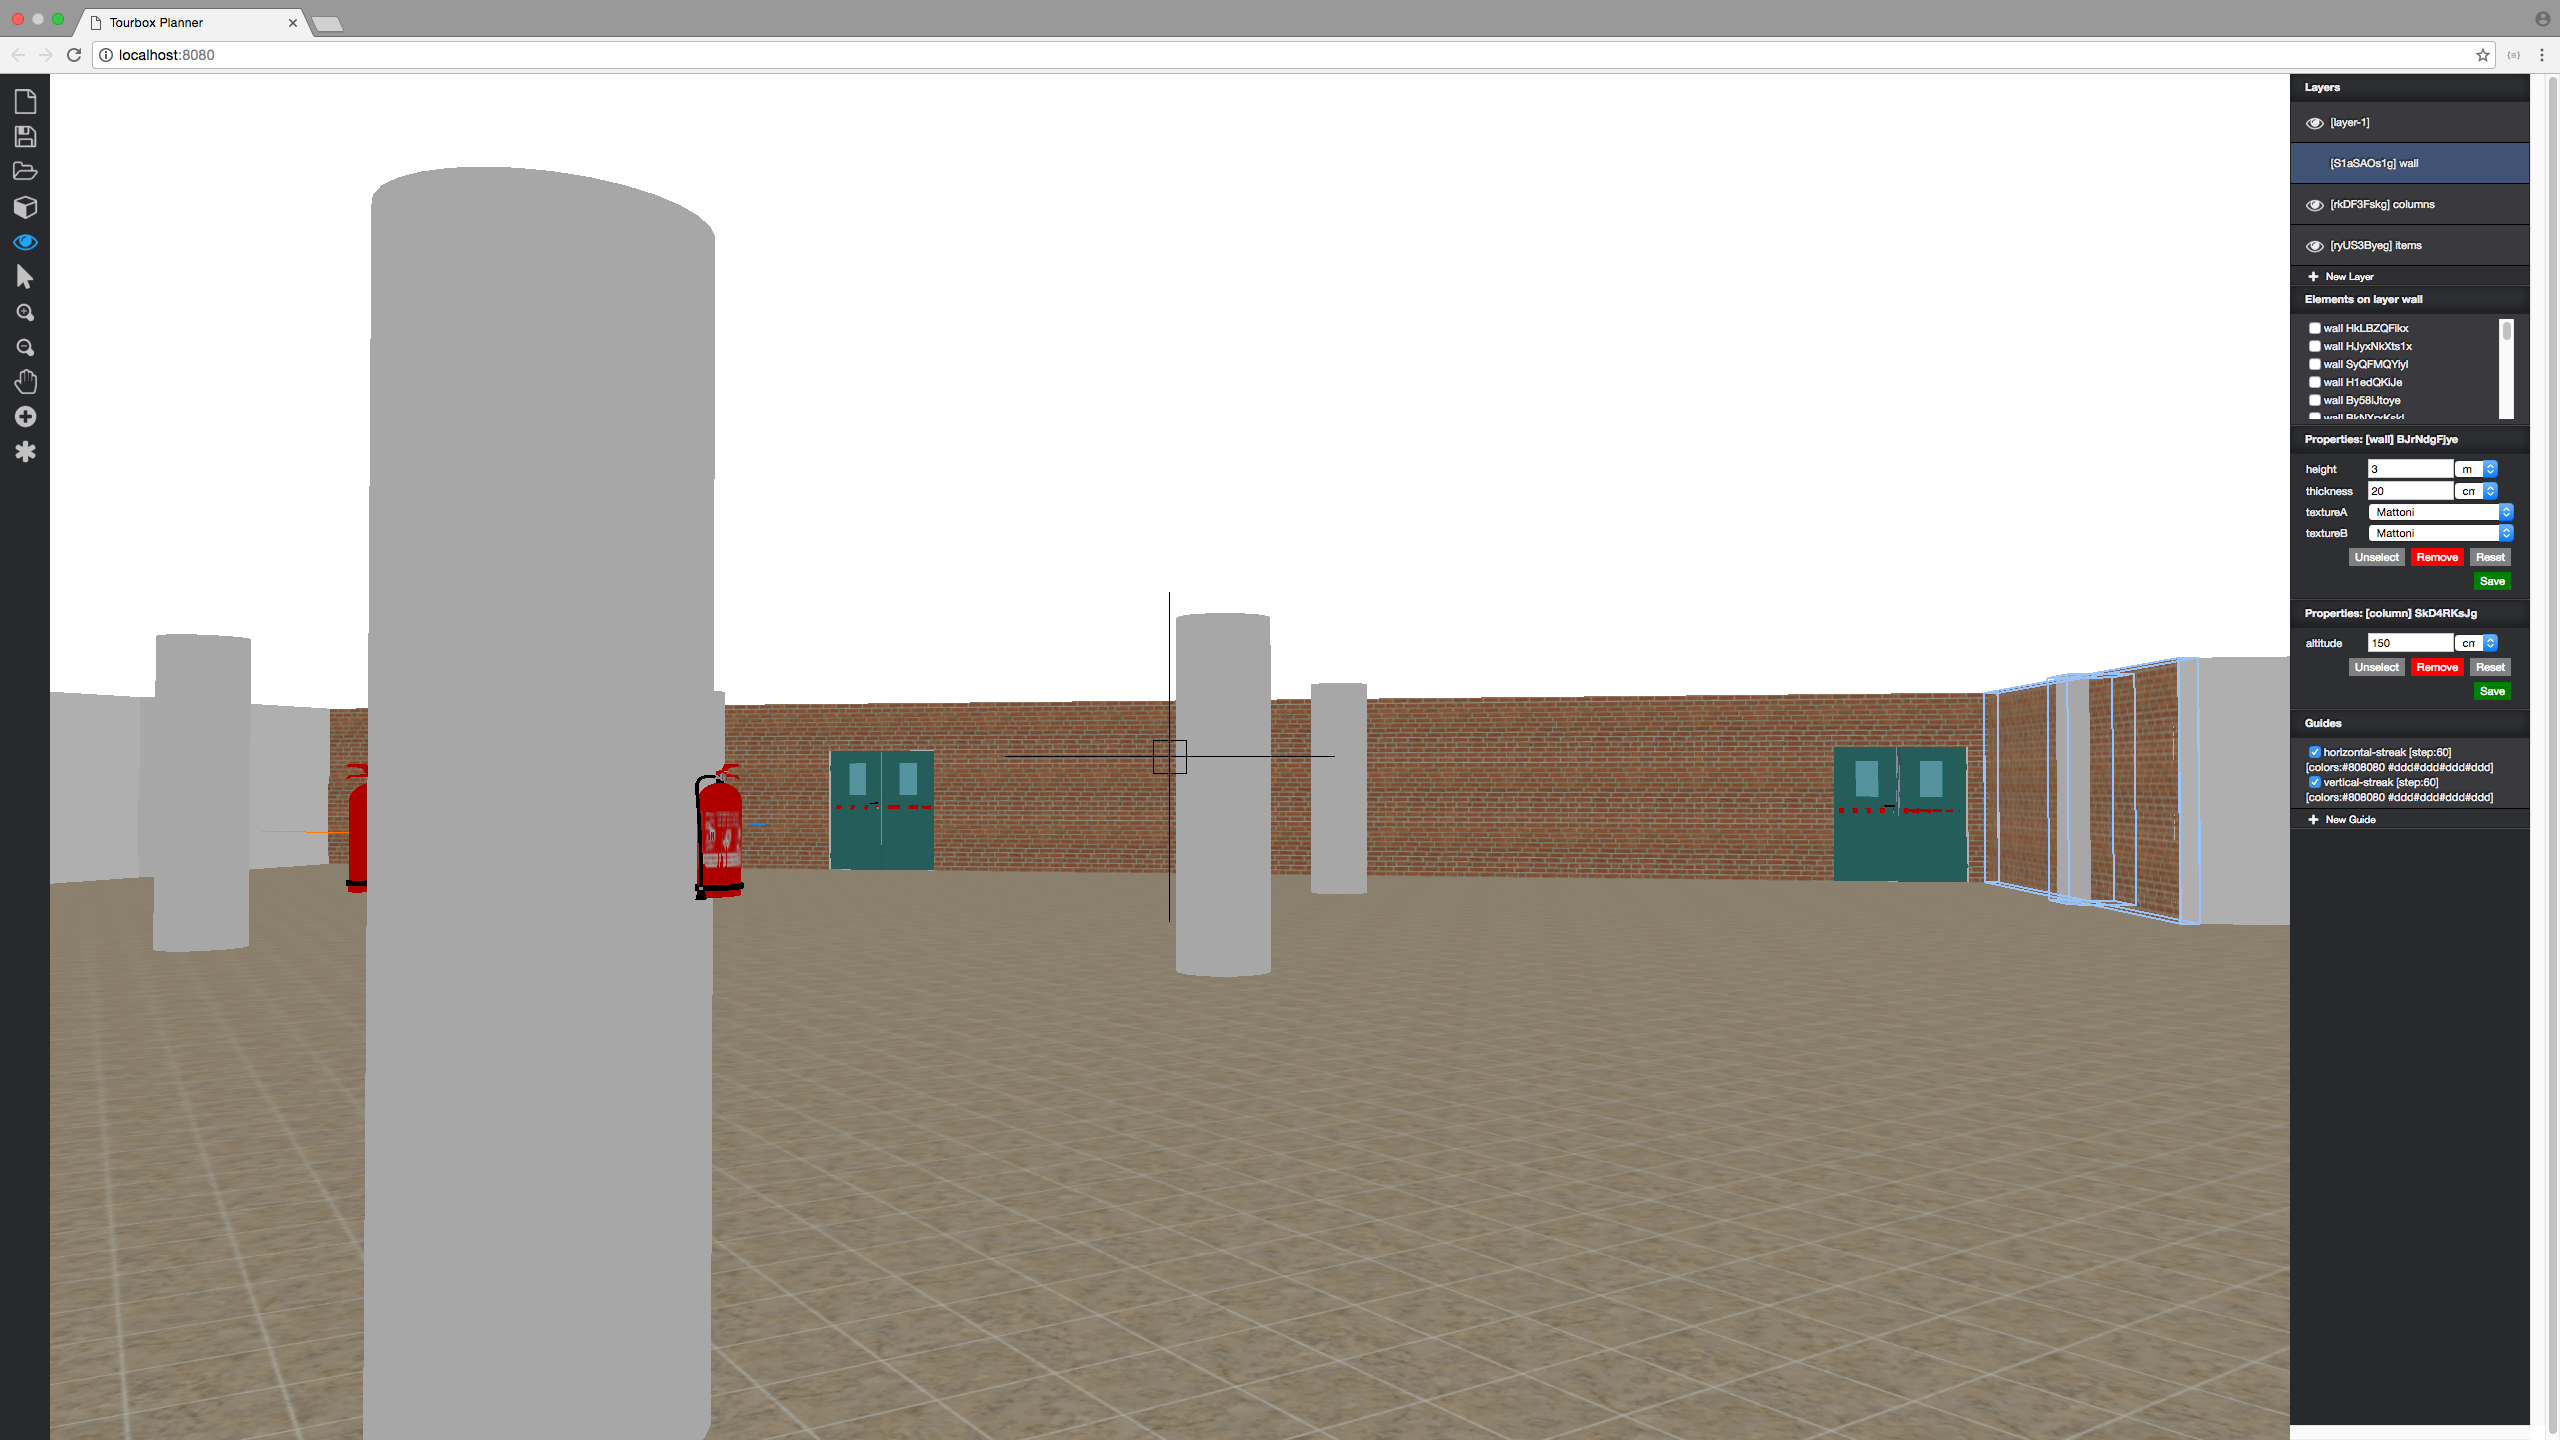
\includegraphics[width=1\linewidth]{images/ui}

   \caption{\emph{Metior} user interface}
   \label{fig:ui}
\end{figure}

\noindent The UI is based on three main areas: \empb{toolbar}, \emph{canvas} and \emph{sidebar}.

\noindent The \emph{toolbar} allow to handle the project life cycle (new, save \& load); to edit the project (showing the plugins catalog, described below); to change the view mode (2D \& 3D); to change the interaction mode (pan \& zoom).

\noindent The canvas shows the project in different view modes:
in the 2D view mode, the projectview from top, it's possible to insert/select elements;
in the 3D view mode, in trackball or first-person mode, using perspective or orthographic camera, it's possible to navigate the project and select elements.

\noindent The sidebar shows the properties of the currently selected element.
In the properties panel it's possible to view the description of the element, to modify any property, or to add/remove metadata.

\subsection{Plugin-architecture}

\noindent The application has been designed to provide a small set of core interaction functionalities and to encapsulate the generation logic for architectural components (from the very basic to the most articulated) into specific plugins.

\noindent A plugin is a software component that can be seamlessy integrated in the system in order to extends its capabilities.
In \emph{Metior}, a plugin represents an architectural element that extends the Building Information Model design.
Technically, a plugin represents a \emph{prototype} (namely a ``class'' in OOP) of a construction element that can be inserted (``instantiated'') in the canvas.

\subsubsection{Definizione di un plugin}

A plugin is described by the following properties:
\begin{itemize}
\item a unique name
\item a description
\item a set of metadata
\item the \emph{occupation type}, that can be one of \emph{linear}, \emph{area} or \emph{volume}
\item the \emph{placement type}, that can be one of \emph{inside} or \emph{over}
\item a set of specific properties relative to the element described
\item a construction function that returns the 2D representation of the element (in SVG format, for the 2D view mode)
\item a construction function that returns the 3D representation of the element (in OBJ format, for the 3D view mode)
\end{itemize}

\subsubsection{Tassonomia dei plugin}\label{ssec:taxonomy}

\noindent The plugins can be organized by the \emph{occupation type} and the \emph{placement type}.

\noindent The \emph{linear} elements extend in one dimension (unless a radial thickness), like hydraulic lines or electrical cables.

\noindent The \emph{area} elements extend in two dimensions (unless a linear thickness), like the separation elements.
They can be divided in \emph{horizontal area}, like floor and ceil, and \emph{vertical area}, like walls.

\noindent The \emph{volume} elements extend in three dimensions.
The can be \emph{fixed volume}, like the piece of furniture, and \emph{scalable volume}, that can be scaled (proportionally or not), like pillars and staircases.

\noindent The \emph{occupation type} determines a different way to instantiate and to insert the element in the canvas.
In particular, in 2D mode, the \emph{linear} elements are inserted drawing lines by drag\&drop;
the \emph{area} elements are inserted drawing the bounding-box of the element by drag\&drop;
the \emph{volume} elements are inserted picking the position of the element by point\&click,
and varying their dimensions modifying the bounding-box by drag\&drop.

\noindent The \emph{placement type} determines if the element can be inserted in the canvas in a specific point occupied or not by other elements.

\noindent The \emph{inside} elements can be inserted in the canvas only inside other elements (that can be \emph{linear}, \emph{area} or \emph{volume}); e.g., a ``window'' is a ``volume inside vertical area'' element,
while an ``hydraulic line'' is a ``linear inside horizontal area'' element.

\noindent The \emph{over} elements can be inserted in the canvas only over other elements (of any type);
e.g., a ``pillar'' is a ``volume over horizontal area'' element,
while an ``electric panel'' is a ``volume over vertical area'' element.

In the design phase, an element that doesn't meet the placement constraints defined by the placement type is notified by the system as a visual warning, showing its bounding-box in semi-transparent blinked red color.

\subsubsection{Propriet� specifiche dei plugin}

\noindent Each plugin has a set of specific properties of the building elements that it represent.
Each property is defined by:
\begin{itemize}
\item a name
\item a type, such as ``number'', ``text'', ``boolean'', o ``custom''
\item a value
\end{itemize}

\noindent According to its type, each property value can be inserted in different ways.
For example, a boolean property value is setted by a checkbox, while a textual property is setted by a text box.
The system lets define new kind of property, defining the component of the user interface that lets insert its value.
For example, a ``color'' property can be introduced defining a UI component composed by three text boxes (one for each RGB color  components), while a ``length'' property can be introduced defining a UI component composed by a text box for the value and a drop-down menu for the unit of measure.

\noindent The specific properties of an element can be edited in the relative panel in the sidebar, once the element is selected in the canvas.


\subsection{Plugin Catalog}
\noindent It is pivotal to provide surveyors with a rich catalog of plugins, to cover all the basic as well as the most advanced modeling requirements. Table~\ref{tab:plugins-example} reports examples of plugins arranged by the introduced taxonomy.

\begin{table}[htbp]
\small
\centering
\begin{tabular}{|
>{\columncolor[HTML]{EFEFEF}}l |l|l|}
\hline
{\color[HTML]{000000} } & \cellcolor[HTML]{EFEFEF}{\color[HTML]{000000} \footnotesize{\bf{inside}}} & \cellcolor[HTML]{EFEFEF}{\color[HTML]{000000} \footnotesize{\bf{over / free}}} \\ \hline
\footnotesize{\bf{linear}}      & \tt{pipe}             & \tt{electrical-conduit}  \\ \hline
\footnotesize{\bf{ver. area}}   & \tt{window, door}     & \tt{wall}                \\ \hline
\footnotesize{\bf{hor. area}}   & \tt{light-panel}      & \tt{ground, ceil}        \\ \hline
\footnotesize{\bf{volume}}      & \tt{pillar}           & \tt{staircase}           \\ \hline
\end{tabular}
\caption{Plugins example according to taxonomy~\ref{ssec:taxonomy}}
\label{tab:plugins-example}
\end{table}

\subsection{Server-side models generation}

\noindent Both 3D and 2D model generation has been designed to be asynchronous: the actual result of the invocation of the generation function is not the model itself but rather a \emph{promise} of the expected result. Such a design is important since the computation for model generation may require a while. In the meantime the user must be able to interact with the interface, which in turn must remain responsive. Relying on this architecture, generation of the models can be easily delegated to a server (as shown in Figure~\ref{fig:c-s-arch}), thus relieving the client from the burden of onerous computations. The server exposes a REST-like HTTP based JSON API to the client. The plugin span from the client to the server since the 2D and 3D generation functions (``3Dgf'' and ``2Dgf'' respectively in Figure~\ref{fig:c-s-arch}) defined by the plugin are actually executed on the server.

\begin{figure}[htbp] %  figure placement: here, top, bottom, or page
   \centering

   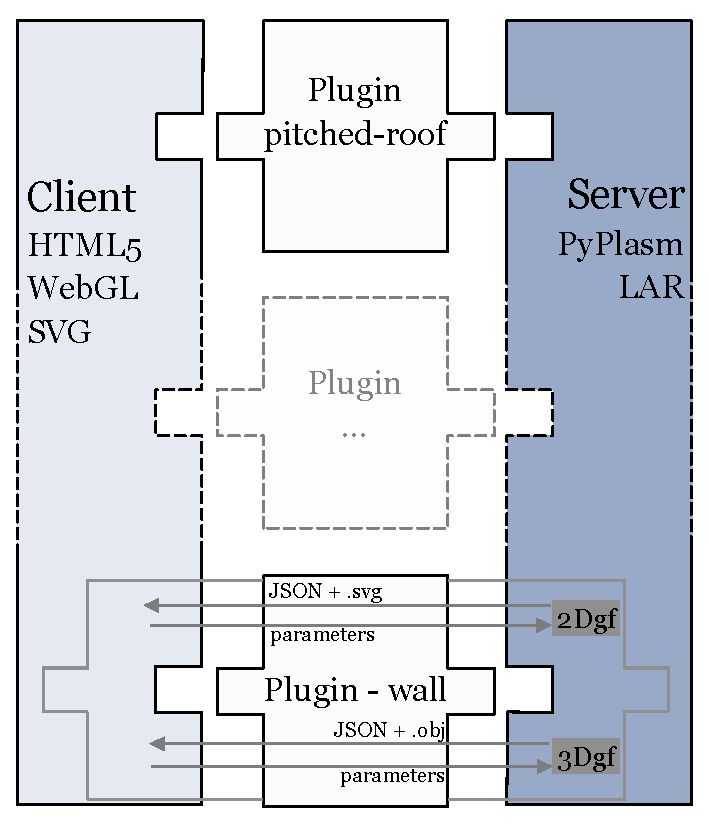
\includegraphics[width=0.6\linewidth]{images/architecture-h}

   \caption{Client/Server architecture for server-side models generation}
   \label{fig:c-s-arch}
\end{figure}

\noindent


